\section{Appendix}

\subsection{Implementation details}
\label{app:method-details}

\paragraph{Partition-tree construction.}
Let the interaction graph of the tensor network be $G=(V,E,w)$, where each node corresponds to one original tensor and edges connect tensors that share internal labels. In the current implementation, edge weights accumulate the dimensions contributed by shared internal labels. On each induced subgraph $G[U]$, we recursively perform a bipartition: if the subgraph is connected, we use a Stoer--Wagner minimum cut to obtain $U_L$ and $U_R$; if the subgraph is degenerate or edgeless, we fall back to a ``single node versus the rest'' split. This process constructs a binary partition tree bottom-up.

\paragraph{Output blocking.}
Let the global open-label order be $\mathcal O=(\ell_1,\ldots,\ell_m)$. In the implementation, only the first $q=\texttt{block\_label\_count}$ open labels are block-partitioned. For each blocked label $\ell_i$, its index set is divided into contiguous chunks of length $\texttt{chunk\_size}$:
\[
I_{\ell_i}^{(1)}, I_{\ell_i}^{(2)}, \ldots.
\]
An output block $\Omega_b$ is then the Cartesian product of the selected local chunks. Blocking is therefore not only a scheduling device for write-back; it also changes the local output dimensions seen by each subtree under the current block.

\paragraph{Local block keys and cross-block caching.}
For a tree node $v$ and output block $\Omega_b$, we define the local block key
\[
\kappa_v(\Omega_b)
=
\left\{
\begin{array}{l}
(\ell, I_{b,\ell}) : \ell \in \mathcal O_v,\\
\ell \text{ is sliced in the current block}
\end{array}
\right\}.
\]
This key retains only the slice constraints visible to subtree $v$ and ignores unrelated block information. The cache key can therefore be written as
\[
K(v,\Omega_b)
=
\bigl(\mathrm{node\_key}(v),\ \kappa_v(\Omega_b),\ \mathrm{sig}(\theta)\bigr),
\]
where $\mathrm{sig}(\theta)$ is the signature of the compression configuration, including rank-selection rules, tolerances, randomized parameters, and optimization strategy. If two global output blocks induce the same $\kappa_v(\Omega_b)$ at node $v$, the cached state can be reused directly.

\paragraph{Root readout.}
At the root, the boundary label set is empty, i.e.,
\[
\mathcal B_{\mathrm{root}}=\varnothing.
\]
The root state therefore degenerates from a general output-side times boundary-side interface into the dense result for the current output block. If the root state is written as $M_{\mathrm{root}} \approx A_{\mathrm{root}} B_{\mathrm{root}}^\top$, the block output is obtained by contracting the final rank dimension.

\paragraph{Exact-contraction baseline.}
The exact baseline (\textsf{exact-TNC}) shares the same tensor-network object and the same output-label order as \method{}. For each output block $\Omega_b$, it directly performs an exact full contraction,
\[
X_{\Omega_b} = \mathrm{contract\_full}(\mathcal N,\Omega_b),
\]
using the exact contraction interface of \texttt{opt\_einsum} under the chosen optimization strategy. Thus, the difference between \method{} and \textsf{exact-TNC} lies primarily in the internal computation path rather than the output interface.

\paragraph{Reproducibility.}
In randomized compression, the current implementation uses a deterministic pseudorandom generator seeded jointly by a base random seed and the state key. As a result, the randomized compression outcome is reproducible for the same network, output block, tree node, and configuration.

\subsection{Experimental details}
\label{app:exp-details}

\paragraph{Network generation.}
The main experiments use Ring-8, Tree-8, Grid $3\times 3$, and Random-8. Tree-8 is generated using a random labeled tree (\texttt{networkx.random\_labeled\_tree}) with $8$ nodes. Random-8 uses an Erd\H{o}s--R\'enyi random graph with a connectedness check (\texttt{networkx.erdos\_renyi\_graph}), again with $8$ nodes and edge probability $p=0.35$. Both are driven by global random seeds $\{0,1,2\}$ in the main experiments.

\paragraph{Tolerance presets.}
Leaf compression and merge compression use separate tolerances $\tau_{\mathrm{leaf}}$ and $\tau_{\mathrm{merge}}$. The three presets used in the strength scan are
\[
\begin{aligned}
\textsf{L1} \quad &(5.0\times10^{-4},\;2.0\times10^{-3}),\\
\textsf{L2} \quad &(1.0\times10^{-3},\;5.0\times10^{-3}),\\
\textsf{L3} \quad &(3.0\times10^{-3},\;1.5\times10^{-2}).
\end{aligned}
\]
In addition, \method{} uses a \texttt{depth\_open}-style schedule in which the local tolerance is adapted as
\[
\tau_{\mathrm{local}}=\tau_{\mathrm{base}}\cdot(1.5)^{\mathrm{depth}}/(\max(1,\mathrm{open\_count}))^{0.5}.
\]

\paragraph{Output-blocking policy.}
All main experiments enable output blocking with \texttt{block\_labels=2} and \texttt{chunk\_size=1}. That is, two open-leg labels are selected as blocking axes and sliced one element at a time, so the full output tensor is contracted and written back block by block.

\paragraph{Timing protocol.}
We use a unified timing protocol with the same task, the same block schedule, and the same stage decomposition for all methods. For each network instance, we first generate the same set of output blocks and then run both \textsf{exact-TNC} and the approximate methods on that schedule. Timing uses a high-resolution clock and accumulates contraction time and emit time separately for every output block, ultimately reporting
\[
T_{\mathrm{total}}=T_{\mathrm{contract}}+T_{\mathrm{emit}}.
\]
We also report $t_{\mathrm{contract}}/t_{\mathrm{total}}$ as a stage-share metric. Speedup is defined as
\[
\mathrm{speedup}=T_{\mathrm{exact\text{-}TNC}}/T_{\mathrm{method}},
\]
and results are aggregated across random seeds $\{0,1,2\}$ to reduce single-run noise.

\subsection{Supplementary visual summary}

\begin{figure*}[t]
\centering
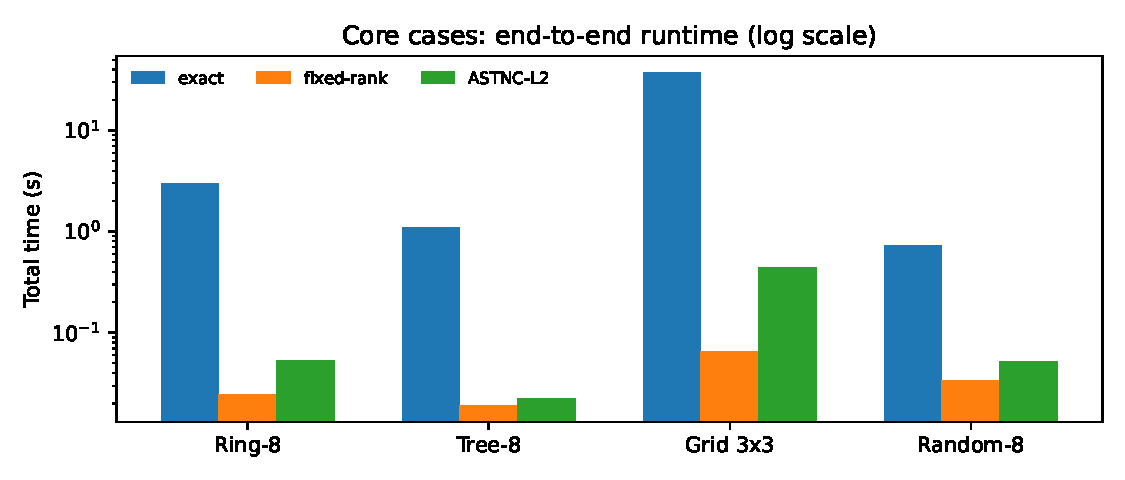
\includegraphics[width=0.92\textwidth]{figures/main_runtime.pdf}
\caption{Supplementary runtime overview across the main benchmark cases. The figure is reused from the original \texttt{paper} assets and can be included directly in an arXiv upload.}
\label{fig:main-runtime}
\end{figure*}

\begin{figure*}[t]
\centering
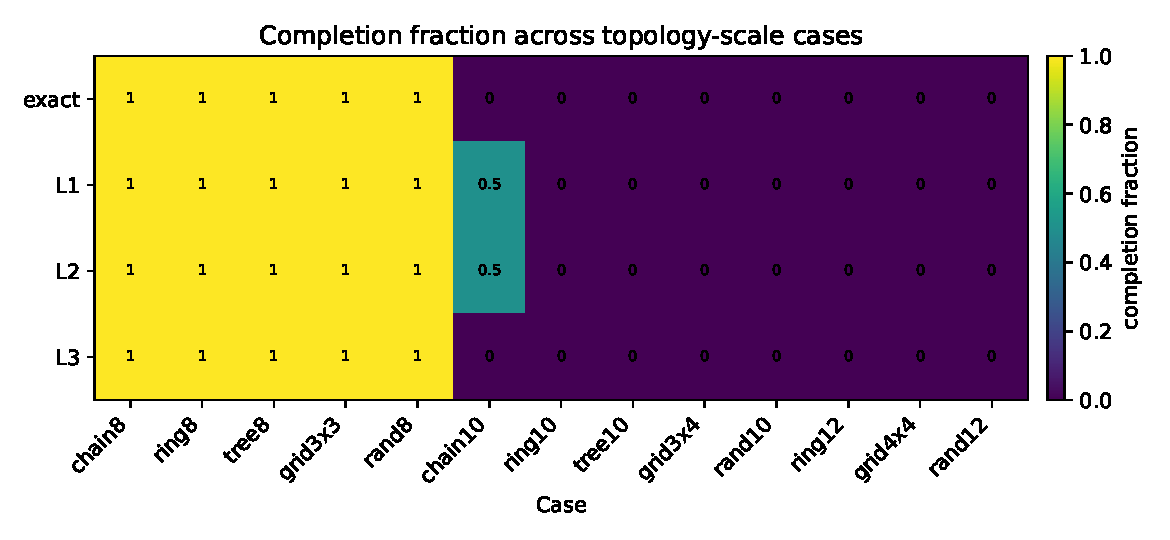
\includegraphics[width=0.92\textwidth]{figures/regime_status.pdf}
\caption{Supplementary regime-status summary across topologies and scales. This figure provides a broader context for the easy, medium, and boundary regimes discussed in the original drafting materials.}
\label{fig:regime-status}
\end{figure*}
